
\section{Studienordnung}
Hier geben wir dir einen Überblick
zur Studien- und Prüfungsordnung an der MLU.
\begin{center}
	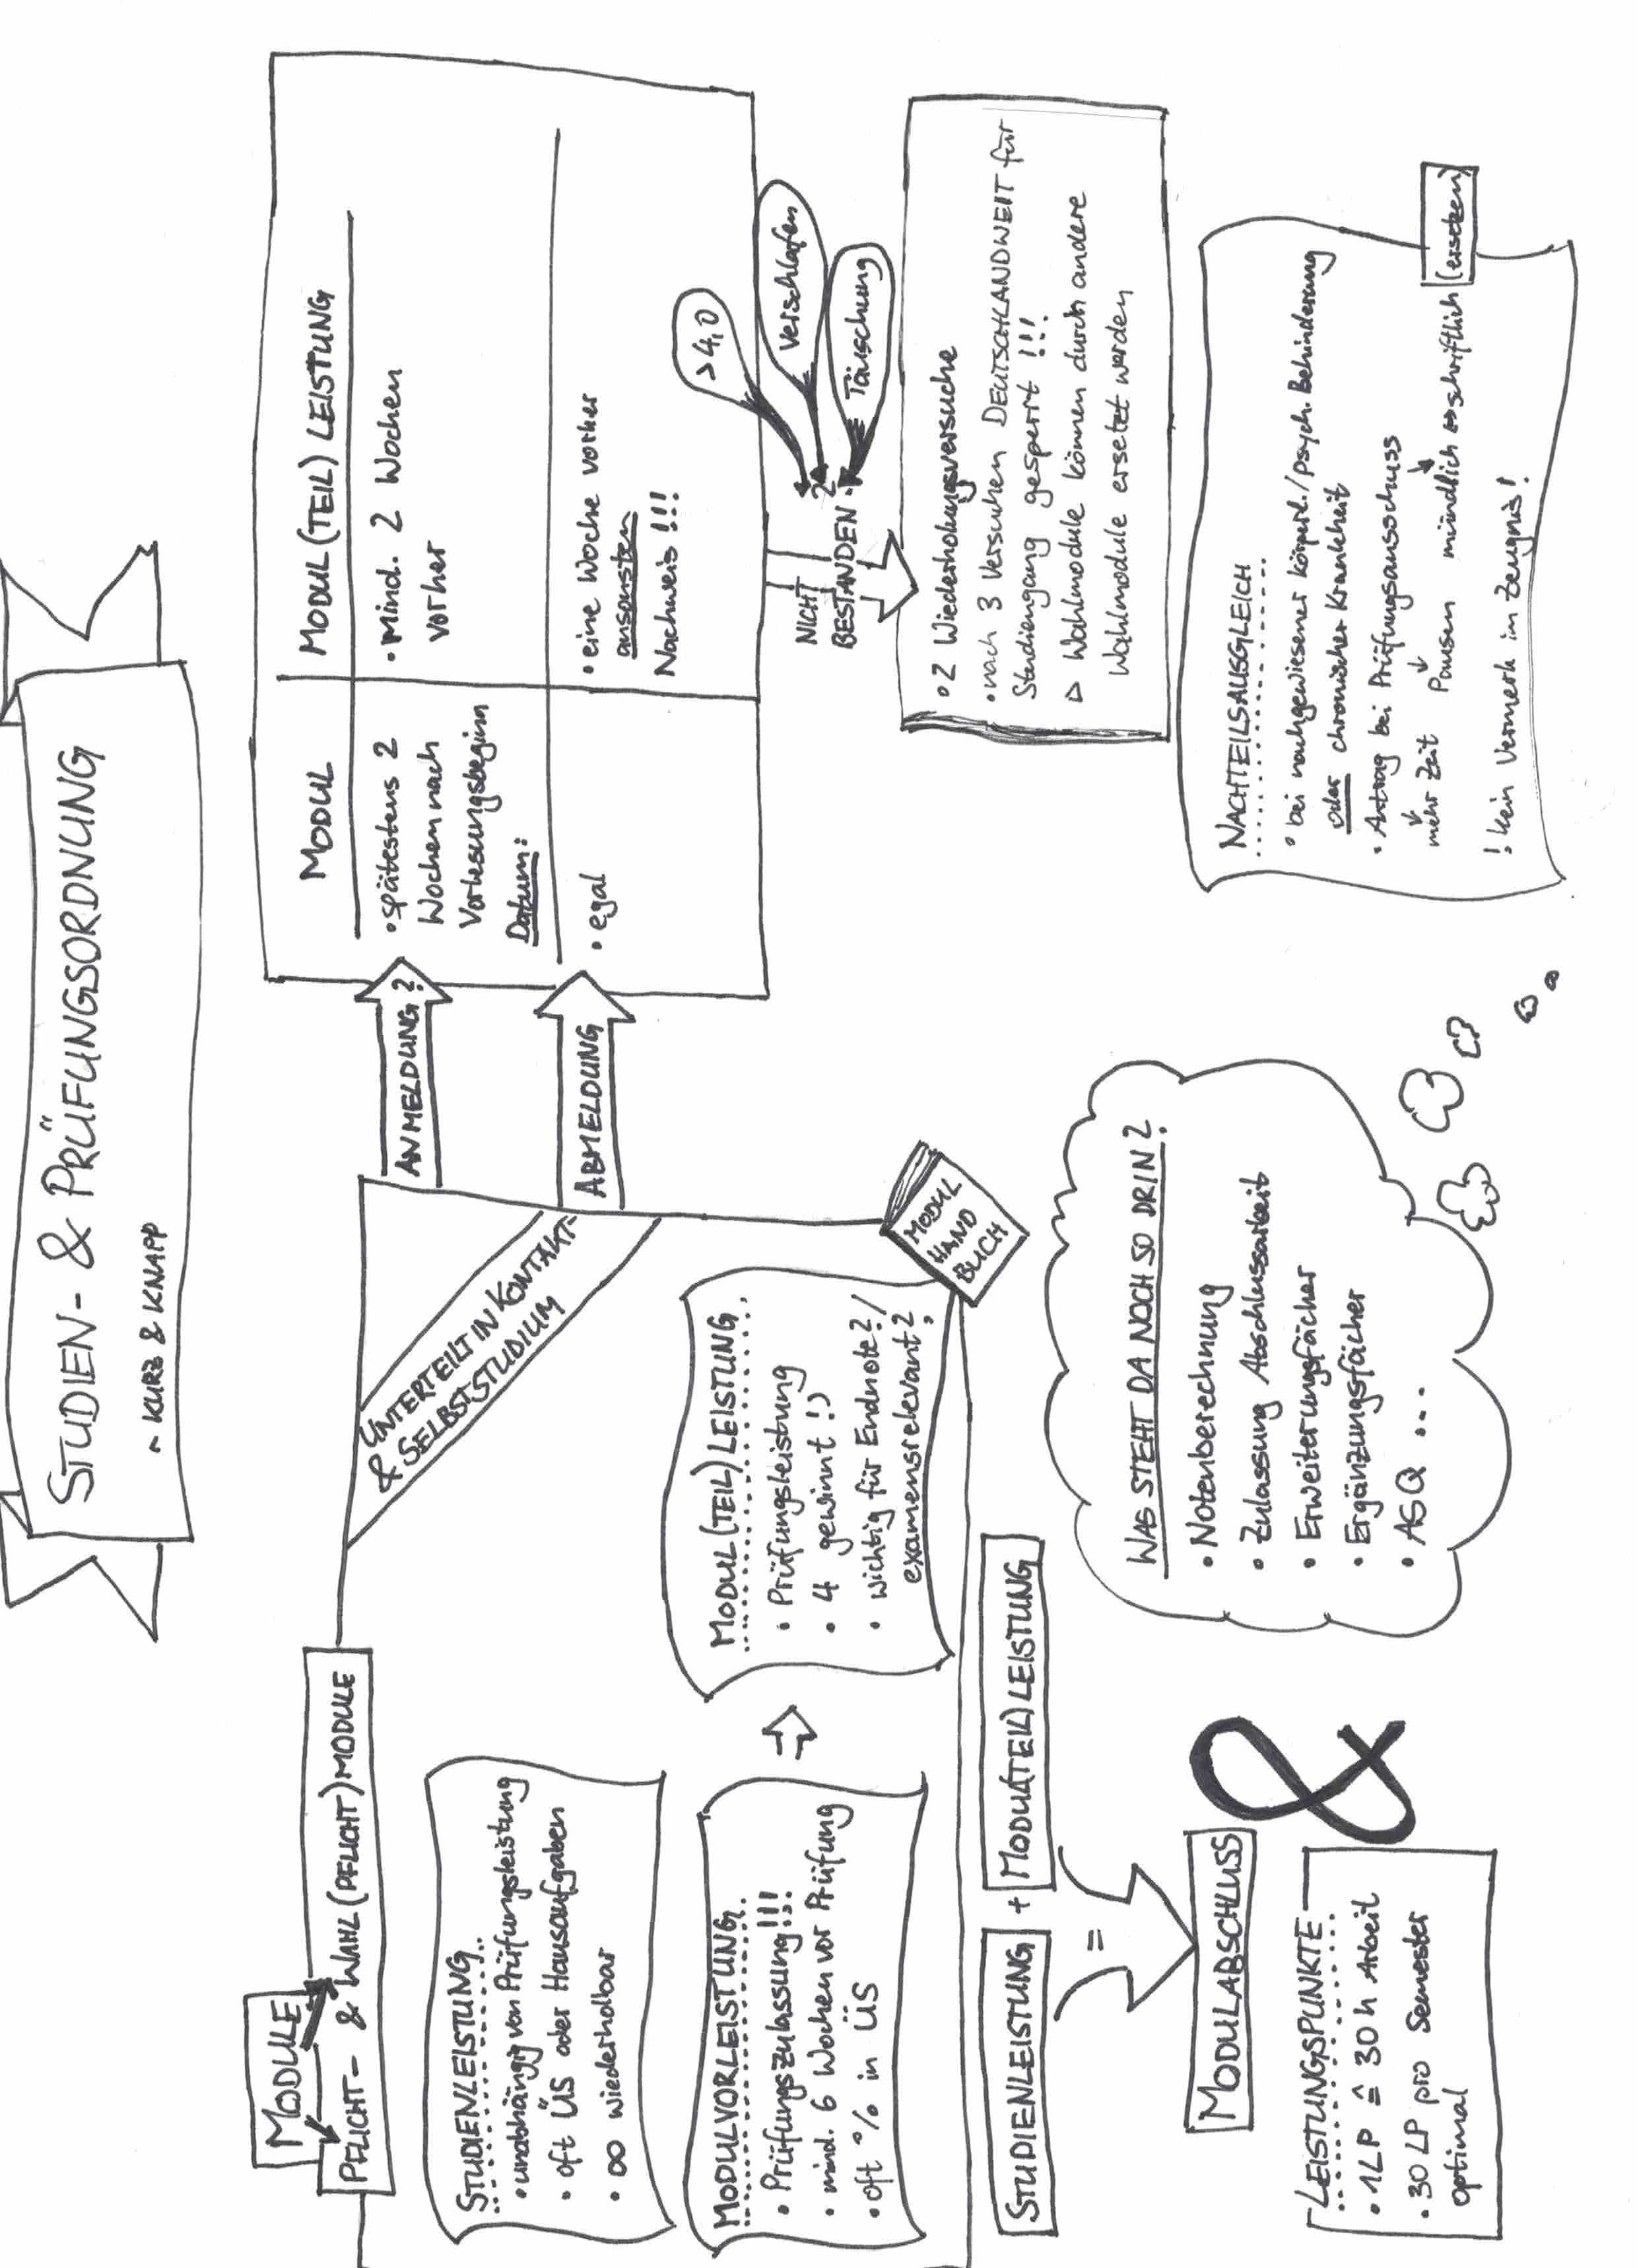
\includegraphics[width=0.89\textwidth]{studiordnung}
\end{center}

\section{Studiengänge}

Im folgenden findet ihr Auszüge aus den Modulhandbüchern und Empfehlungen aus den Regelstudienplänen, außerdem Ansprechpartner für Fragen und \textquote{Sonderwünsche}.
Fragen können immer auch an den FSR gerichtet werden.

\subsection{Studienberater}
\subsubsection{Mathematik/Wirtschaftsmathematik}
Dr.\ Hans-Georg Rackwitz \\
Theodor-Lieser-Str.~5, Raum~127 \\
Telefon: +49\,345\,55\,24608\\
E-Mail: \email{hans-georg.rackwitz@mathematik.uni-halle.de}\\

\subsubsection{Informatik/Bioinformatik}
Dr.\ Steffen Schüler \\
Von-Seckendorff-Platz~1, Raum~4.20 \\
Telefon: +49\,345\,55\,24735 \\
E-Mail: \email{steffen.schueler@informatik.uni-halle.de}

\subsubsection{Lehramt}
Zentrum für Lehrerbildung \\
Dr. Marie-Theres Müller \\
Dachritzstraße~12, Raum~205 \\
Telefon: +49\,345\,55\,21717 \\
E-Mail: \email{zlb@uni-halle.de}

\newpage

\section{Studiengangsübersichten}

\subsection{Informatik}
\label{studiengang_informatik}

\subsubsection{Regelstudienplan}
\begin{singlespace}
	\begin{small}
		\begin{longtabu} to \textwidth {X|r@{\hspace{0.75em}}r@{\hspace{0.75em}}r@{\hspace{0.75em}}r@{\hspace{0.75em}}r@{\hspace{0.75em}}r|r}
			\toprule
			\textbf{Modul}&\multicolumn{6}{l|}{\textbf{LP pro Semester}}&\textbf{LP}\\
			& 1. & 2. & 3. & 4. & 5. & 6. &\\
			\midrule
			\endfirsthead
			\midrule
			\textbf{Modul}&\multicolumn{6}{l|}{\textbf{LP pro Semester}}&\textbf{LP}\\
			& 1. & 2. & 3. & 4. & 5. & 6. &\\
			\midrule
			\endhead
			\midrule
			\endfoot
			\bottomrule
			\endlastfoot
			\multicolumn{8}{l}{\textbf{Informatik-Grundlagen}} \\
			Objektorientierte Programmierung & 5 & & & & & & 5 \\ 
			Einführung in die Rechnerarchitektur & 5 & & & & & & 5 \\ 
			Mathematische Grundlagen der Informatik \& Konzepte der Modellierung & 7 & 8 & & & & & 15 \\ 
			Einführung in Betriebssysteme & & 5 & & & & & 5 \\ 
			Einführung in die technische Informatik & & 5 & & & & & 5 \\ 
			Datenstrukturen \& effiziente Algorithmen~I & & 5 & & & & & 5 \\ 
			Konzepte der Programmierung & & & 5 & & & & 5 \\ 
			Automaten \& Berechenbarkeit & & & & 10 & & & 10 \\
			\midrule
			\multicolumn{8}{l}{\textbf{Mathematik}} \\
			Diskrete Strukturen, lineare Algebra \& Analysis (Mathe B) & 8 & 7 & & & & & 15 \\ 
			Einführung in Data Science & & & & 5 & & & 5 \\
			\midrule
			\multicolumn{8}{l}{\textbf{Informatik-Vertiefung}} \\
			Einführung in Datenbanken & & & 5 & & & & 5 \\ 
			Datenstrukturen \& effiziente Algorithmen~II & & & 5 & & & & 5 \\ 
			Softwaretechnik & & & 5 & & & & 5 \\ 
			Einführung in die Bildverarbeitung & & & 5 & & & & 5 \\
			Projektpraktikum & & & & 5 & 10 & & 15 \\ 
			Einführung in die Rechnernetze \& verteilte Systeme & & & & & 5 & & 5 \\  
			Gestaltung \& Durchführung von Fachvorträgen in der Informatik & & & & & 5 & & 5 \\
			\midrule
			\multicolumn{8}{l}{\textbf{Anwendungsfach, ASQ, Wahlpflicht}} \\
			Allgemeine Schlüsselqualifikationen (ASQ) & 5 & & & & & 5 & 10 \\
			Anwendungsfach & & & 5 & 5 & 5 & & 15 \\ 
			„Spezialisierung“\,/\,Wahlpflicht & & & & 5 & 5 & 10 & 20 \\ 
			\midrule
			\textbf{Bachelorarbeit} & & & & & & 15 & 15 \\
		\end{longtabu}
	\end{small}
\end{singlespace}

\subsection{Bioinformatik}
\label{studiengang_bioinformatik}

\subsubsection{Regelstudienplan}
\begin{singlespace}
	\begin{small}
		\begin{longtabu} to \textwidth {X|r@{\hspace{0.75em}}r@{\hspace{0.75em}}r@{\hspace{0.75em}}r@{\hspace{0.75em}}r@{\hspace{0.75em}}r|r}
			\toprule
			\textbf{Modul}&\multicolumn{6}{l|}{\textbf{LP pro Semester}}&\textbf{LP}\\
			& 1. & 2. & 3. & 4. & 5. & 6. &\\
			\midrule
			\endfirsthead
			\midrule
			\textbf{Modul}&\multicolumn{6}{l|}{\textbf{LP pro Semester}}&\textbf{LP}\\
			& 1. & 2. & 3. & 4. & 5. & 6. &\\
			\midrule
			\endhead
			\midrule
			\endfoot
			\bottomrule
			\endlastfoot
			\multicolumn{8}{l}{\textbf{Pflichtbereich Informatik}}\\ 
			Objektorientierte Programmierung & 5 & & & & & & 5 \\
			Grundlagen der Bioinformatik & 8 & 7 & & & & & 15 \\ 
			Datenstrukturen \& effiziente Algorithmen~I & & 5 & & & & & 5 \\ 
			Enführung in Datenbanken & & & 5 & & & & 5 \\ 
			Softwaretechnik & & & 5 & & & & 5 \\ 
			Algorithmen auf Sequenzen~I & & & & 5 & & & 5 \\ 
			Spezielle Probleme der Bioinformatik & & & & 5 & & & 5 \\ 
			Gestaltung \& Durchführung von Fachvorträgen in der Bioinformatik & & & & & 5 & & 5 \\
			Statistische Datenanalyse \& Maschinelles Lernen in der Bioinformatik~I & & & & & 5 & & 5 \\ 
			\midrule
			\multicolumn{8}{l}{\textbf{Pflichtbereich Mathematik}}\\ 
			Diskrete Strukturen, lineare Algebra \& Analysis (Mathe B) & 7 & 8 & & & & & 15 \\ 
			Einführung in Data Science & & & & 5 & & & 5 \\ 
			\midrule
			\multicolumn{8}{l}{\textbf{Pflichtbereich Biologie}}\\ 
			Biologie für Bioinformatiker~I (Zellbiologie, Botanik) & 8 & & & & & & 8 \\ 
			Biologie für Bioinformatiker~II (Mikrobiologie, Ökologie) & & 7 & & & & & 7 \\ 
			Biologie für Bioinformatiker~III (Genetik, Zoologie) & & & 10 & & & & 10 \\ 
			\midrule
			\multicolumn{8}{l}{\textbf{Pflichtbereich Biochemie}}\\
			Allgemeine Biochemie für Bioinformatiker & & & 10 & & & & 10 \\ 
			\midrule
			\multicolumn{8}{l}{\textbf{Pflichtbereich Chemie}}\\ 
			Organische Chemie im Nebenfach (OC-N) & 2 & 3 & & & & & 5 \\ 
			Physikalische Chemie für die Bioinformatik (PC-N~VI) & & & & 5 & & & 5 \\ 
			\midrule
			\multicolumn{8}{l}{\textbf{Pflichtbereich ASQ/Wahlpflicht}}        \\ 
			Allgemeine Schlüsselqualifikationen & & & & 5 & 5 & & 10 \\ 
			Wahlpflicht* & & & & 5 & 15 & 15 & 35 \\ 
			\midrule
			\textbf{Bachelorarbeit} & & & & & & 15 & 15 \\
		\end{longtabu}
	\end{small}
\end{singlespace}
Von den mit * markierten Wahlpflichtmodulen müssen jeweils mindestens 10~LP aus den Bereichen Informatik und Biowissenschaften erbracht werden.

\subsection{Informatik Lehramt}
\label{studiengang_infolehramt}

\subsubsection{Regelstudienplan}

\begin{singlespace}
	\begin{small}
		\begin{longtabu} to \textwidth {X|l|r}
			\toprule
			\textbf{Modul} & \textbf{Semester} & \textbf{LP} \\
			\midrule
			\endfirsthead
			\midrule
			\textbf{Modul} & \textbf{Semester} & \textbf{LP} \\
			\midrule
			\endhead
			\midrule
			\endfoot
			\bottomrule
			\endlastfoot
			\multicolumn{3}{l}{\textbf{Pflichtmodule Informatik}}\\
			Objektorientierte Programmierung & 1. & 5 \\
			Einführung in Rechnerarchitektur & 1. & 5 \\
			Mathematische Grundlagen der Informatik \& Konzepte der Modellierung & 1.\,--\,2. & 15 \\
			Datenstrukturen \& effiziente Algorithmen I & 2.\,/\,4. & 5 \\
			Technische Informatik, Betriebssysteme \& Rechnernetze (Lehramt) & 3. & 5 \\
			Konzepte der Programmierung & 3. & 5 \\
			Einführung in Datenbanken & 3.\,/\,5. & 5 \\
			Datenbank-Programmierung & 4.\,/\,6. & 5 \\
			Automaten \& Berechenbarkeit* & 4.\,/\,6. & 10 \\
			Softwaretechnik (Lehramt) & 5. & 5 \\
			Informatik \& Gesellschaft & \(\geq\) 5. & 5 \\
			\midrule
			\multicolumn{3}{l}{\textbf{Wahlmodule Informatik}}\\
			Wahlmodul I & \(\geq\) 5. & 5 \\
			Wahlmodul II* & \(\geq\) 5. & 5 \\
			\midrule
			\multicolumn{3}{l}{\textbf{Fachdidaktik Informatik}}\\
			Didaktik der Informatik AB & 3.\,/\,4. & 5 \\
			Didaktik der Informatik CDE & \(\geq\) 4. & 5 \\
			Didaktik der Informatik FG & \(\geq\) 5. & 5 \\
		\end{longtabu}
	\end{small}
\end{singlespace}
Die mit * gekennzeichnete Module sind nur von LAGs zu belegen.

\subsection{Mathematik}
\label{studiengang_mathematik}

\subsubsection{Regelstudienplan}

\begin{singlespace}
	\begin{small}
		\begin{longtabu} to \textwidth {X|r@{\hspace{0.75em}}r@{\hspace{0.75em}}r@{\hspace{0.75em}}r@{\hspace{0.75em}}r@{\hspace{0.75em}}r|r}
			\toprule
			\textbf{Modul}&\multicolumn{6}{l|}{\textbf{LP pro Semester}}&\textbf{LP}\\
			& 1. & 2. & 3. & 4. & 5. & 6. &\\
			\midrule
			\endfirsthead
			\midrule
			\textbf{Modul}&\multicolumn{6}{l|}{\textbf{LP pro Semester}}&\textbf{LP}\\
			& 1. & 2. & 3. & 4. & 5. & 6. &\\
			\midrule
			\endhead
			\midrule
			\endfoot
			\bottomrule
			\endlastfoot
			\multicolumn{3}{l}{\textbf{Pflichtbereich}}\\
			Objektorientierte Programmierung & 5 & & & & & & 5\\
			Analysis~I\,\&\,II & 9 & 9 & & & & & 18\\
			Lineare Algebra & 9 & 9 & & & & & 18\\
			Datenstrukturen \& effiziente Algorithmen~I & & 5 & & & & & 5\\
			Numerik~I\,\&\,II & & 9 & 9 & & & & 18\\
			Algebra & & & 9 & & & & 9\\
			Analysis~III & & & 9 & & & & 9\\
			Praktikum & & & & 6 & & & 6\\
			Maßtheorie & & & & 8 & & & 8\\
			Wahrscheinlichkeitstheorie \& Statistik & & & & 8 & & & 8\\
			Fachseminar & & & & & 5 & & 5\\
			Funktionalanalysis & & & & & 8 & & 8\\
			\midrule
			\multicolumn{3}{l}{\textbf{Wahlpflichtbereich}}\\
			Anwendungsfach & 5 & & & 5 & & 10 & 20\\
			Proseminar & & & 3 & & & & 3\\
			Allgemeine Schlüsselqualifikationen & & & & 5 & & 5 & 10\\
			Vertiefung Mathematik & & & & & 15 & & 15\\
			\midrule
			\textbf{Bachelorarbeit}& & & & & & 15 & 15\\
		\end{longtabu}
	\end{small}
\end{singlespace}

\subsection{Wirtschaftsmathematik}
\label{studiengang_wima}

\subsubsection{Regelstudienplan}

Die Wirtschaftswissenschaftsmodule sind Platzhalter für die unter der Tabelle aufgeführten Wahlpflichtmodule.

\begin{singlespace}
	\begin{small}
		\begin{longtabu} to \textwidth {X|r@{\hspace{0.75em}}r@{\hspace{0.75em}}r@{\hspace{0.75em}}r@{\hspace{0.75em}}r@{\hspace{0.75em}}r|r}
			\toprule
			\textbf{Modul}&\multicolumn{6}{l|}{\textbf{LP pro Semester}}&\textbf{LP}\\
			& 1. & 2. & 3. & 4. & 5. & 6. &\\
			\midrule
			\endfirsthead
			\midrule
			\textbf{Modul}&\multicolumn{6}{l|}{\textbf{LP pro Semester}}&\textbf{LP}\\
			& 1. & 2. & 3. & 4. & 5. & 6. &\\
			\midrule
			\endhead
			\midrule
			\endfoot
			\bottomrule
			\endlastfoot
			\multicolumn{8}{l}{\textbf{Pflichtbereich}}\\
			Objektorientierte Programmierung & 5 & & & & & & 5\\
			Analysis~I\,\&\,II & 9 & 9 & & & & & 18\\
			Lineare Algebra & 9 & 9 & & & & & 18\\
			Datenstrukturen \& effiziente Algorithmen~I & & 5 & & & & & 5\\
			Optimierung & & 10 & 10 & & & & 20\\
			Analysis~III & & & 9 & & & & 9\\
			Maßtheorie & & & & 8 & & & 8\\
			Numerik für Wirtschaftsmathematiker & & & & 8 & & & 8\\
			Praktikum & & & & 8 & & & 8\\
			Wahrscheinlichkeitstheorie \& Statistik & & & & 8 & & & 8\\
			Fachseminar & & & & & 5 & & 5\\
			Versicherungsmathematik \& Risikotheorie & & & & & 8 & & 8\\
			\midrule
			\multicolumn{3}{l}{\textbf{Wahlpflichtbereich}}\\
			ASQ & 5 & & & & & 5 & 10\\
			Vertiefung Informatik & & & 5 & & & & 5\\
			Vertiefung Wirtschaftswissenschaften & & & 5 & & 10 & 10 & 25\\
			Vertiefung Mathematik & & & & & 5 & & 5\\
			\midrule
			\textbf{Bachelorarbeit}& & & & & & 15 & 15\\
		\end{longtabu}
	\end{small}
\end{singlespace}

\subsection{Mathematik Lehramt}
\label{studiengang_lehramt}

\subsubsection{Regelstudienplan Gymnasium}
\label{studiengang_lag}

Bei den mit * gekennzeichneten Teilgebieten muss jeweils nur ein Modul besucht werden.

\begin{singlespace}
	\begin{small}
		\begin{longtabu} to \textwidth {X|l|r}
			\toprule
			\textbf{Modul} & \textbf{Semester} & \textbf{LP} \\
			\midrule
			\endfirsthead
			\midrule
			\textbf{Modul} & \textbf{Semester} & \textbf{LP} \\
			\midrule
			\endhead
			\midrule
			\endfoot
			\bottomrule
			\endlastfoot
			Analysis~I \& II & 1.\,--\,2. & 15\\
			Lineare Algebra & 1.\,--\,2. & 15\\
			Wahrscheinlichkeitstheorie \& Statistik & 4.\,/\,6. & 6\\
			Proseminar & \(\geq\) 3. & 5\\
			Grundlagen der numerischen Mathematik & \(\geq\) 3. & 5\\
			Algebra & \(\geq\) 3. & 7\\
			Fachseminar & \(\geq\) 5. & 5\\
			Vertiefungsmodul (nur wenn Erstfach)& \(\geq\) 3.& 5\\
			Mathematikdidaktik~I & 3.\,--\,4. & 5\\
			Mathematikdidaktik~II & 4.\,--\,5. & 5\\
			Mathematikdidaktik~III & 6.\,--\,7. & 5\\
			\midrule
			\multicolumn{3}{l}{\textbf{Wahlpflichtbereich Geometrie*}}\\
			Geometrie & 5.\,/\,7. & 7\\
			Differentialgeometrie & 5.\,/\,7. & 7\\
			\midrule
			\multicolumn{3}{l}{\textbf{Wahlpflichtbereich Grundlagen*}}\\
			Geschichte der Mathematik & \(\geq\) 4.& 5\\
			Grundlagen der Mathematik & \(\geq\) 4.& 5\\
			\midrule
			\multicolumn{3}{l}{\textbf{Wahlpflichtbereich Analysis/Numerik*}}\\
			Funktionentheorie & \(\geq\) 5.& 5\\
			Gewöhnliche Differentialgleichungen& \(\geq\) 5.& 5\\
			Theorie \& Numerik gewöhnlicher Dgl.& \(\geq\) 5.& 5\\
		\end{longtabu}
	\end{small}
\end{singlespace}

\subsubsection{Regelstudienplan Sekundarschule}
\label{studiengang_las}

Bei dem mit * gekennzeichneten Teilgebiet müssen zwei Module besucht werden.

\begin{singlespace}
	\begin{small}
		\begin{longtabu} to \textwidth {X|l|r}
			\toprule
			\textbf{Modul} & \textbf{Semester} & \textbf{LP} \\
			\midrule
			\endfirsthead
			\midrule
			\textbf{Modul} & \textbf{Semester} & \textbf{LP} \\
			\midrule
			\endhead
			\midrule
			\endfoot
			\bottomrule
			\endlastfoot
			Lineare Algebra & 1.\,--\,2. & 15\\
			Elemente der Mathematik & 1.\,--\,2. & 5\\
			Analysis~I & 3.& 10\\
			Elemente der Kombinatorik \& Stochastik & 3.\,/\,5. & 5\\
			Elemente der Geometrie & 3.\,/\,5. & 5\\
			Proseminar & 3.\,--\,6. & 5 \\
			Algebra & 3.\,/\,5. & 5\\
			Vertiefungsmodul (nur wenn Erstfach)& 4.\,--\,8. & 5\\
			Mathematikdidaktik~I & 3.\,--\,4. & 5\\
			Mathematikdidaktik~II & 4.\,--\,5. & 5\\
			Mathematikdidaktik~III & 6.\,--\,7. & 5\\
			\midrule
			\multicolumn{3}{l}{\textbf{Wahlpflichtbereich Mathematik*}}\\
			Analysis~II & 4.\,/\,6.  & 5\\
			Geschichte der Mathematik & 4.\,/\,6.  & 5\\
			Grundlagen der numerischen Mathematik & 5.\,/\,7.  & 5\\
			Funktionentheorie & 5.\,/\,7. & 5\\
			Geometrie & 5.\,/\,7. & 5\\
			Diskrete Mathematik & 5.\,/\,7. & 5\\
		\end{longtabu}
	\end{small}
\end{singlespace}
